\documentclass{beamer}
\usepackage[utf8]{inputenc}
\mode<presentation> {

\usetheme{Madrid}
}

\usepackage{graphicx} 
\usepackage{booktabs}
\usepackage{tikz}
\usepackage{eurosym}

\setbeamertemplate{navigation symbols}{}

\title[PAS]{Approches mathématiques pour l'optimisation du placement des conteneurs dans la cour de stockage des terminaux portuaires du Port Autonome de Strasbourg} % The short title appears at the bottom of every slide, the full title is only on the title page

\author[SEME]{Beaude Laurence\textsuperscript{1}
\and 
Caldini-Queiros Céline\textsuperscript{2}
\and 
Hild Romain\textsuperscript{2}
\and 
Maassarani Mohamad\textsuperscript{2}
\and 
Maumy-Bertrand Myriam\textsuperscript{2}
\and
Sala Lorenzo\textsuperscript{2}} % Your name
\institute[]{1: Universit\'e C\^ote d'Azur, CNRS, INRIA COFFEE, 
  Laboratoire J.A. Dieudonn\'e,\\
2: Université de Strasbourg, IRMA}
\date[16/11/18]{Semaine d'Etude Math-Entreprise\\
16 novembre 2018} % Date, can be changed to a custom date

\begin{document}

\begin{frame}
\titlepage % Print the title page as the first slide
\end{frame}


\begin{frame}
\frametitle{Overview} % Table of contents slide, comment this block out to remove it
\tableofcontents % Throughout your presentation, if you choose to use \section{} and \subsection{} commands, these will automatically be printed on this slide as an overview of your presentation
\end{frame}

%----------------------------------------------------------------------------------------
%	PRESENTATION SLIDES
%----------------------------------------------------------------------------------------

%------------------------------------------------

\section{Présentation du port}

\begin{frame}{Le terminal à conteneurs sud}
  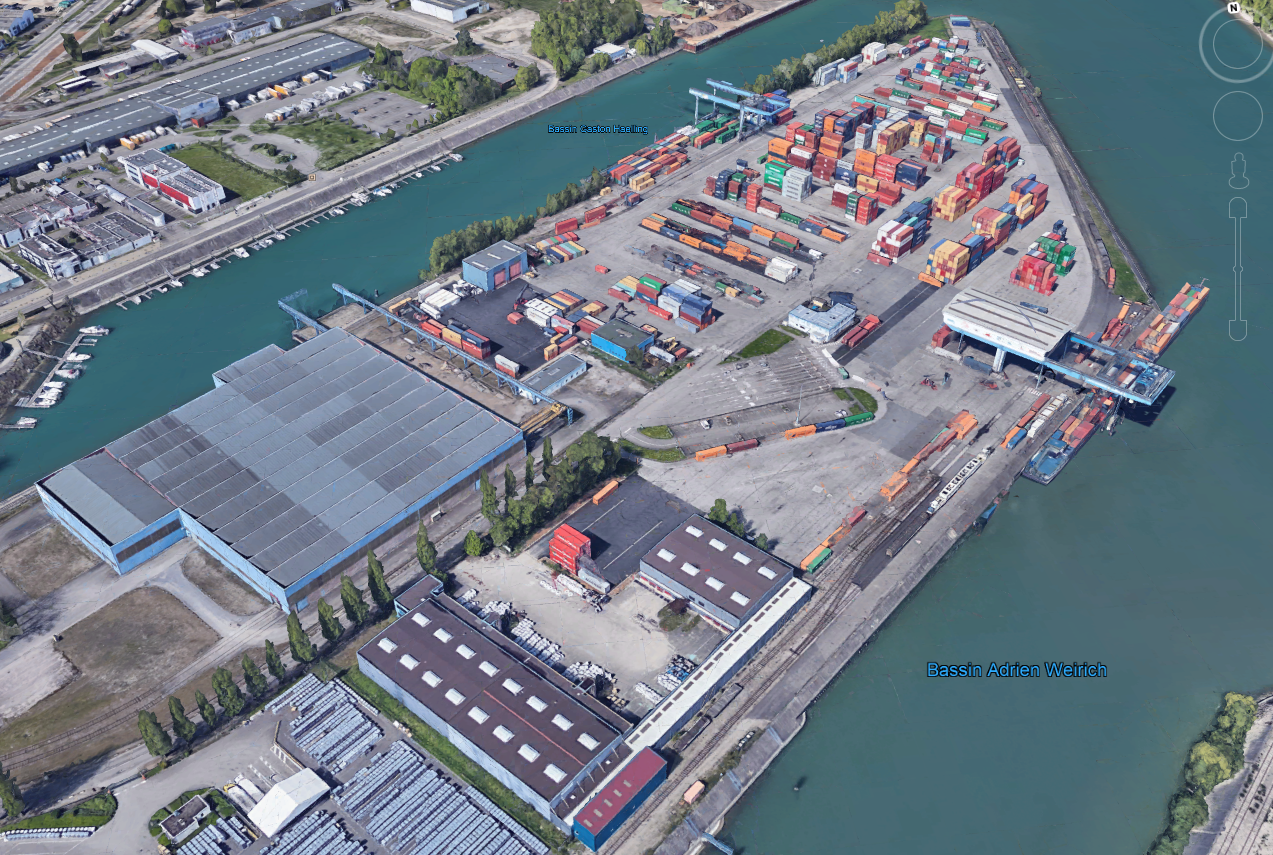
\includegraphics[width=\textwidth]{../images/image14}
\end{frame}

\begin{frame}{Le terminal à conteneurs sud}
  \begin{itemize}
  \item Infrastructures et outillage
    \begin{itemize}
    \item
      2 portiques fluviaux à conteneurs, mobiles
    \item
      1 portique fluvial à colis lourds (capacité 460 tonnes)
    \item
      1 420 mètres de linéaire ferroviaire en 4 voies de longueur variant entre 330 et 400 mètres
    \item
      8 reach-stackers
    \item
      itinéraires routiers adaptés aux colis lourds
    \item
      systèmes informatiques intégrés (TOS)
    \item
      superficie : 10 ha
    \end{itemize}
  \item Enjeux
    \begin{itemize}
    \item Congestion de poids lourds
    \item Elargissement sur un terrain adjacent pour améliorer la fluidité des trafics
    \end{itemize}
  \end{itemize}
\end{frame}

\begin{frame}{Problèmatique du PAS}
  \begin{itemize}
  \item 3000 conteneurs sur le site
  \item 500 entrées/sorties par jour
  \item aucune visibilité sur la date de sortie des conteneurs
  \item politique du First In, First Out
  \end{itemize}
\end{frame}

\section{Problématique et modèle}

\begin{frame}{Contraintes sur la géométrie}
  \vfill 
  \begin{itemize}
  \item $N_t$ : largeur de la travée $t$.
  \end{itemize} 
  \vfill
  Contraintes : 
  \vfill
  \begin{itemize}
  \item $1 \leq N_t \leq 15$,
    \vfill
  \item $\mathrm{Card}(N_t\vert N_t \leq  6) \geq  P$,
    \vfill
  \item la largeur d'une allée est supérieure à $15m$.
    \vfill
  \end{itemize}   
  \vfill
\end{frame}

\begin{frame}{Génération de la configuration}
  \begin{itemize}
  \item Dynamique \cite{rekik2015}:
    \begin{itemize}
    \item Prend en compte les événements aléatoire en temps-réel
    \item On se place dans le cas statique où les événements sont déterminés
    \end{itemize}
    \vfill
  \item Définition détaillée des coûts \cite{kim98}:
    \begin{itemize}
    \item Prend en compte les coûts fixes d'un emplacement, d'une grue/stacker
    \item Prend en compte les coûts variables pour un remaniement,...
    \end{itemize}
    \vfill
  \item Optimisation de forme \cite{allaire2006}:
    \begin{itemize}
    \item Essayer d'écrire le problème et les contraintes en un problème continu
    \item Utilisation de level set
    \end{itemize}
  \end{itemize}
\end{frame}

\begin{frame}{Génération de la configuration}
  \begin{itemize}
  \item Génétique \cite{gotteland2004}:
    \begin{itemize}
    \item Configuration de départ, opérations admises et critère de décision
    \item Gestion du parc d'avion dans un aéroport 
    \end{itemize}
    \vfill
  \item Heuristique \cite{ndiaye2015}:
    \begin{itemize}
    \item Test de configurations possibles
    \end{itemize}
    \vfill
  \item Combinatoire \cite{moussi2012}:
    \begin{itemize}
    \item Création d'une grille et remplissage conteneurs/allées
    \item Test de toutes les configurations admissibles
    \end{itemize}
    \vfill
  \item Geometrical and functional layout optimization \cite{jacquenot2010}:
    \begin{itemize}
    \item Algorithmes sur le placement d'objets
    \end{itemize}
  \end{itemize}
\end{frame}

\begin{frame}{Algorithme}
  \resizebox{\textwidth}{!}{
  \begin{tikzpicture}%[scale=0.2]
    \draw (0,0) node[draw,rectangle,text width=4cm,align=center,fill=blue!20] {Génération de la configuration};
    \draw (6,0) node[draw,rectangle,text width=4cm,align=center,fill=blue!20] {Calcul du coût};
    \draw (11,0) node[draw,diamond,fill=red!10]{Optimal?};
    \draw (14,0) node[draw,rectangle,fill=green!30]{Fin};
    \draw[->,thick] (2.1,0) -- (3.9,0);
    \draw[->,thick] (8.1,0) -- (9.8,0);
    \draw[->,thick] (12.2,0) -- (13.6,0);
    \draw (12.9,0) node[above] {Oui};
    \draw[->,thick] (2.1,0) -- (3.9,0);
    \draw[->,thick] (11,1.2) -- (11,3) -- (0,3) -- (0,0.55);
    \draw (5.5,3) node[above] {Non};
  \end{tikzpicture}}
  \vfill
  \emph{Objectif : } minimiser la fonction coût en fonction de la \emph{géométrie} et de la \emph{configuration}.
  \vfill
  L'idéal serait de pouvoir générer des géométries et des configurations, puis de comparer les différentes valeurs des fonctions coût. 
  \vfill  
\end{frame}

\begin{frame}{Hypothèses}
  \begin{itemize}
  \item On se concentre sur le cas des conteneurs vides
    \vfill
  \item On ne considère que le nouveau portique
    \vfill
  \item On se concentre sur la zone entre les camions et le nouveau portique
    \vfill
  \item On ne considère que les itinéraires bateau-stockage-camion
    \vfill
  \item Les conteneurs sont stockés par blocs de hauteur 5
    \vfill
  \item Ils sont déchargés dans une travée par une allée et sont chargés par l'allée à l'autre bout de la travée
    \vfill
  \item Les travées ne contiennent des conteneurs appartenant à un seul client
    \vfill
  \item On ne considère que des conteneurs de taille identique (20 pieds).
  \end{itemize}
  \vfill
\end{frame}

\begin{frame}{Fonction de coût}
  \vfill
  La fonction coût sert à comparer les différentes configurations, c'est-à-dire la géométrie et la répartition des clients dans les travées.\\
  \vfill
  La fonction coût cherche à évaluer les coûts moyens liés aux emplacements des 4500 EVP présent en moyenne dans le port.
  Cette fonction coût tient compte des déplacements entrée-sortie en fonction de la fréquence de déplacement des conteneur qui peut dépendre de chaque client.
  \vfill
  On attribue donc un poids à chaque catégorie (client+dimension), représentant la probabilité que les travées attribuées à cette catégorie soient visitées.
\end{frame}

\begin{frame}{Fonction de coût}
  La fonction coût correspond à la distance moyenne parcourue par un conteneur.
  \begin{description}
  \item[$d_t$] distance associée à une travée $t$ pour une géométrie fixée.
  \item[$\mu_c$] poids du client $c$,
  \item[$x_{t,c}$] nombre d'emplacements utilisés par le client dans la travée $t$.
  \end{description}
  \vfill
  La fonction coût  : 
  $$ F(t_c)=\sum_t \sum_c d_t\mu_c x_{t,c}.  $$
  \vfill
\end{frame}

\begin{frame}{Poids des clients}
  Extraits à partir de données fournies sur 2 mois : 
  \vfill
  \begin{description}
  \item[$V_{tot}$] nombre total de mouvements de conteneurs sur le port,
  \item[$V_c$] nombre de mouvements de conteneurs par le client $c$.
  \end{description}
  \vfill
  Le poids du client est donné par:
  \begin{equation*}
    \mu_c = \frac{V_c}{V_{tot}}
  \end{equation*}
\end{frame} 

\section{Résultats et perspectives}

\begin{frame}{Coût de la configuration actuelle}
  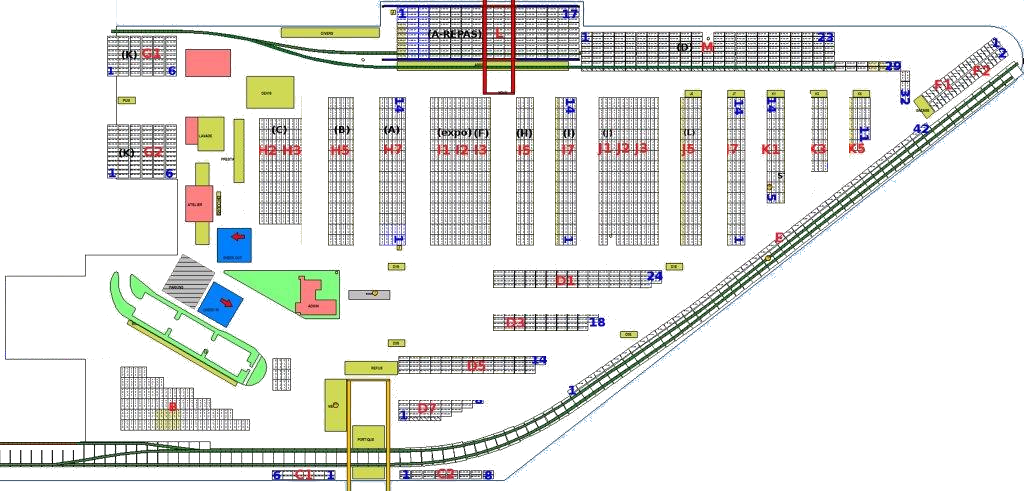
\includegraphics[width=\textwidth]{../images/Plan_Terminal.png}
  \vfill
  \begin{itemize}
  \item conteneurs: capacité occupée/totale = 4500/4850
  \item emplacements: capacité occupée/totale = 900/970
  \item travées: capacité occupée/totale = 126/144
  \end{itemize}
  \vfill
  \begin{center}
    Coût = 762.45
  \end{center}
\end{frame}

\begin{frame}{Coût d'une possible configuration}
  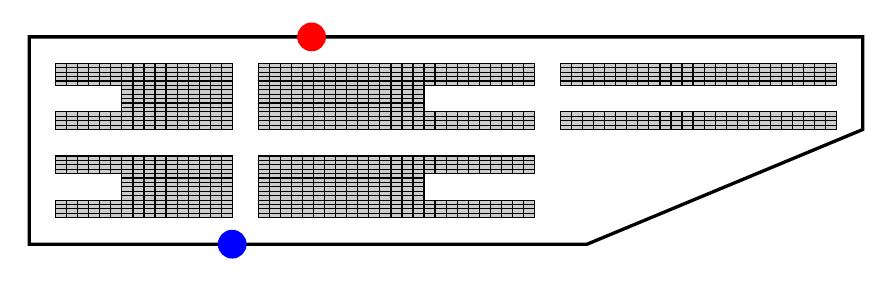
\begin{tikzpicture}[scale=0.07]
%\draw[help lines] (0,0) grid (142,-28);
\colorlet{Grey}{black!20}
%% External perimeter of the harbour
\draw[very thick] (0,0) -- (151.2,0)
	-- (151.2,-16.8) -- (151.2-50,-37.6)
	-- (0,-37.6) -- cycle;
%% Zone top left
\def\a{4.8}
\def\b{-4.8}
\draw[fill=Grey] (\a,\b) -- (\a+32,\b)
	-- (\a+32,\b-12) -- (\a,\b-12)
	-- (\a,\b-12+3.2) -- (\a+12,\b-12+3.2)
	-- (\a+12,\b-4) -- (\a,\b-4) -- cycle;
%
\foreach \x in {0,...,5}
{
	\draw[thin] (\a+2*\x,\b) -- (\a+2*\x,\b-0.8*5);
	\draw[thin] (\a+2*\x,\b-12) -- (\a+2*\x,\b-12+0.8*4);
	\draw[thin] (\a,\b-0.8*\x) -- (\a+32,\b-0.8*\x);
}
\foreach \x in {0,...,10}
{
	\draw[thin] (\a+12+2*\x,\b) -- (\a++12+2*\x,\b-0.8*15);
}
\foreach \x in {0,...,4}
	{\draw[thin] (\a,\b-4-4.8-0.8*\x) -- (\a+32,\b-4-4.8-0.8*\x);}
\foreach \x in {0,...,6}
	{\draw[thin] (\a+12,\b-4-0.8*\x) -- (\a+32,\b-4-0.8*\x);}
%%%%%%%%%%%%%%		
%% Zone bottom left %%
%%%%%%%%%%%%%%
\def\a{4.8}
\def\b{-21.6}
\draw[fill=Grey] (\a,\b) -- (\a+32,\b)
-- (\a+32,\b-11.2) -- (\a,\b-11.2)
-- (\a,\b-11.2+3.2) -- (\a+12,\b-11.2+3.2)
-- (\a+12,\b-3.2) -- (\a,\b-3.2) -- cycle;
%
\foreach \x in {0,...,5}
{
	\draw[thin] (\a+2*\x,\b) -- (\a+2*\x,\b-0.8*4);
	\draw[thin] (\a+2*\x,\b-11.2) -- (\a+2*\x,\b-11.2+0.8*4);
}
\foreach \x in {0,...,10}
{
	\draw[thin] (\a+12+2*\x,\b) -- (\a+12+2*\x,\b-0.8*14);
}
\foreach \x in {0,...,4}
{
	\draw[thin] (\a,\b-3.2-4.8-0.8*\x) -- (\a+32,\b-3.2-4.8-0.8*\x);
	\draw[thin] (\a,\b-0.8*\x) -- (\a+32,\b-0.8*\x);
}
\foreach \x in {0,...,6}
	{\draw[thin] (\a+12,\b-3.2-0.8*\x) -- (\a+32,\b-3.2-0.8*\x);}
%%%%%%%%%%%%%%
%% Zone top central %%
%%%%%%%%%%%%%%
\def\a{41.6}
\def\b{-4.8}
\draw[fill=Grey] (\a,\b) -- (\a+50,\b)
	-- (\a+50,\b-4) -- (\a+50-20,\b-4)
	-- (\a+50-20,\b-4-4.8) -- (\a+50,\b-4-4.8)
	-- (\a+50,\b-12) -- (\a,\b-12) -- cycle;
%
\foreach \x in {0,...,15}
{
	\draw[thin] (\a+2*\x,\b) -- (\a+2*\x,\b-0.8*15);
	\draw[thin] (\a,\b-0.8*\x) -- (\a+30,\b-0.8*\x);
}
\foreach \x in {0,...,10}
{
	\draw[thin] (\a+30+2*\x,\b) -- (\a+30+2*\x,\b-0.8*5);
	\draw[thin] (\a+30+2*\x,\b-8.8) -- (\a+30+2*\x,\b-8.8-0.8*4);
}
\foreach \x in {0,...,5} {\draw[thin] (\a+30,\b-0.8*\x) -- (\a+50,\b-0.8*\x);}
\foreach \x in {0,...,4} {\draw[thin] (\a+30,\b-8.8-0.8*\x) -- (\a+50,\b-8.8-0.8*\x);}
%%%%%%%%%%%%%%%%
%% Zone bottom central %%
%%%%%%%%%%%%%%%%
\def\a{41.6}
\def\b{-21.6}
\draw[fill=Grey] (\a,\b) -- (\a+50,\b)
-- (\a+50,\b-3.2) -- (\a+50-20,\b-3.2)
-- (\a+50-20,\b-3.2-4.8) -- (\a+50,\b-3.2-4.8)
-- (\a+50,\b-11.2) -- (\a,\b-11.2) -- cycle;
%
\foreach \x in {0,...,4} {
	\draw[thin] (\a+30,\b-0.8*\x) -- (\a+50,\b-0.8*\x);
	\draw[thin] (\a+30,\b-8-0.8*\x) -- (\a+50,\b-8-0.8*\x);
}
\foreach \x in {0,...,10}
{
	\draw[thin] (\a+30+2*\x,\b) -- (\a+30+2*\x,\b-0.8*4);
	\draw[thin] (\a+30+2*\x,\b-8) -- (\a+30+2*\x,\b-8-0.8*4);
}
\foreach \x in {0,...,15} {\draw[thin] (\a+2*\x,\b) -- (\a+2*\x,\b-0.8*14);}
\foreach \x in {0,...,14} {	\draw[thin] (\a,\b-0.8*\x) -- (\a+30,\b-0.8*\x);}
%%%%%%%%%%%%%%%%
%%%% Zone top right %%%%
%%%%%%%%%%%%%%%%
\def\a{41.6+4.8+50}
\def\b{-4.8}
\draw[fill=Grey] (\a,\b) -- (\a+50,\b)
-- (\a+50,\b-4) -- (\a,\b-4) -- cycle;
\draw[fill=Grey] (\a,\b-4-4.8) -- (\a+50,\b-4-4.8) 
	-- (\a+50,\b-4-4.8) -- (\a+50,\b-12) -- (\a,\b-12) -- cycle;
%
\foreach \x in {0,...,25} {
	\draw[thin] (\a+2*\x,\b) -- (\a+2*\x,\b-0.8*5);
	\draw[thin] (\a+2*\x,\b-8.8) -- (\a+2*\x,\b-8.8-0.8*4);
}
\foreach \x in {0,...,5} {\draw[thin] (\a,\b-0.8*\x) -- (\a+50,\b-0.8*\x);}
\foreach \x in {0,...,4} {\draw[thin] (\a,\b-8.8-0.8*\x) -- (\a+50,\b-8.8-0.8*\x);}
%% Bateau
%\draw (46.4+4.8,0) circle[radius=5pt];
\node[mark size=5pt,color=red] at (46.4+4.8,0) {\pgfuseplotmark{*}};
%% Camion
\node[mark size=5pt,color=blue] at (4.8+32,-37.6) {\pgfuseplotmark{*}};
\end{tikzpicture}
  \vfill
  \begin{itemize}
  \item conteneurs: capacité occupée/totale = 4865/6110
  \item emplacements: capacité occupée/totale = 973/1222
  \item travees: capacité occupée/totale = 108/164
  \end{itemize}
  \vfill
  \begin{center}
    {\color{green!50!black}Coût = 465.497}
  \end{center}
\end{frame}

\begin{frame}{Conclusion}
  \uncover<1->{
  \begin{exampleblock}{Conclusion}
    \begin{itemize}
    \item Définition d'une fonction de coût pour une configuration
    \item Exemple de calcul du coût pour deux configurations
    \item Liste d'algorithme de génération de configuration
    \end{itemize}
  \end{exampleblock}
}
\uncover<2->{
  \begin{alertblock}{Perspectives}
    \begin{itemize}
    \item Cadre plus général
    \item Algorithme de génération de configuration
    \item Amélioration du calcul du poids par catégorie
    \end{itemize}
  \end{alertblock}}
\end{frame}








%----------------------------------------------------------------------------------------

\end{document}